\documentclass[11pt,preprint, authoryear]{elsarticle}

\usepackage{lmodern}
%%%% My spacing
\usepackage{setspace}
\setstretch{1.2}
\DeclareMathSizes{12}{14}{10}{10}

% Wrap around which gives all figures included the [H] command, or places it "here". This can be tedious to code in Rmarkdown.
\usepackage{float}
\let\origfigure\figure
\let\endorigfigure\endfigure
\renewenvironment{figure}[1][2] {
    \expandafter\origfigure\expandafter[H]
} {
    \endorigfigure
}

\let\origtable\table
\let\endorigtable\endtable
\renewenvironment{table}[1][2] {
    \expandafter\origtable\expandafter[H]
} {
    \endorigtable
}


\usepackage{ifxetex,ifluatex}
\usepackage{fixltx2e} % provides \textsubscript
\ifnum 0\ifxetex 1\fi\ifluatex 1\fi=0 % if pdftex
  \usepackage[T1]{fontenc}
  \usepackage[utf8]{inputenc}
\else % if luatex or xelatex
  \ifxetex
    \usepackage{mathspec}
    \usepackage{xltxtra,xunicode}
  \else
    \usepackage{fontspec}
  \fi
  \defaultfontfeatures{Mapping=tex-text,Scale=MatchLowercase}
  \newcommand{\euro}{€}
\fi

\usepackage{amssymb, amsmath, amsthm, amsfonts}

\def\bibsection{\section*{References}} %%% Make "References" appear before bibliography


\usepackage[round]{natbib}

\usepackage{longtable}
\usepackage[margin=2.3cm,bottom=2cm,top=2.5cm, includefoot]{geometry}
\usepackage{fancyhdr}
\usepackage[bottom, hang, flushmargin]{footmisc}
\usepackage{graphicx}
\numberwithin{equation}{section}
\numberwithin{figure}{section}
\numberwithin{table}{section}
\setlength{\parindent}{0cm}
\setlength{\parskip}{1.3ex plus 0.5ex minus 0.3ex}
\usepackage{textcomp}
\renewcommand{\headrulewidth}{0.2pt}
\renewcommand{\footrulewidth}{0.3pt}

\usepackage{array}
\newcolumntype{x}[1]{>{\centering\arraybackslash\hspace{0pt}}p{#1}}

%%%%  Remove the "preprint submitted to" part. Don't worry about this either, it just looks better without it:
\makeatletter
\def\ps@pprintTitle{%
  \let\@oddhead\@empty
  \let\@evenhead\@empty
  \let\@oddfoot\@empty
  \let\@evenfoot\@oddfoot
}
\makeatother

 \def\tightlist{} % This allows for subbullets!

\usepackage{hyperref}
\hypersetup{breaklinks=true,
            bookmarks=true,
            colorlinks=true,
            citecolor=blue,
            urlcolor=blue,
            linkcolor=blue,
            pdfborder={0 0 0}}


% The following packages allow huxtable to work:
\usepackage{siunitx}
\usepackage{multirow}
\usepackage{hhline}
\usepackage{calc}
\usepackage{tabularx}
\usepackage{booktabs}
\usepackage{caption}


\newenvironment{columns}[1][]{}{}

\newenvironment{column}[1]{\begin{minipage}{#1}\ignorespaces}{%
\end{minipage}
\ifhmode\unskip\fi
\aftergroup\useignorespacesandallpars}

\def\useignorespacesandallpars#1\ignorespaces\fi{%
#1\fi\ignorespacesandallpars}

\makeatletter
\def\ignorespacesandallpars{%
  \@ifnextchar\par
    {\expandafter\ignorespacesandallpars\@gobble}%
    {}%
}
\makeatother

\newlength{\cslhangindent}
\setlength{\cslhangindent}{1.5em}
\newenvironment{CSLReferences}%
  {\setlength{\parindent}{0pt}%
  \everypar{\setlength{\hangindent}{\cslhangindent}}\ignorespaces}%
  {\par}


\urlstyle{same}  % don't use monospace font for urls
\setlength{\parindent}{0pt}
\setlength{\parskip}{6pt plus 2pt minus 1pt}
\setlength{\emergencystretch}{3em}  % prevent overfull lines
\setcounter{secnumdepth}{5}

%%% Use protect on footnotes to avoid problems with footnotes in titles
\let\rmarkdownfootnote\footnote%
\def\footnote{\protect\rmarkdownfootnote}
\IfFileExists{upquote.sty}{\usepackage{upquote}}{}

%%% Include extra packages specified by user

%%% Hard setting column skips for reports - this ensures greater consistency and control over the length settings in the document.
%% page layout
%% paragraphs
\setlength{\baselineskip}{12pt plus 0pt minus 0pt}
\setlength{\parskip}{12pt plus 0pt minus 0pt}
\setlength{\parindent}{0pt plus 0pt minus 0pt}
%% floats
\setlength{\floatsep}{12pt plus 0 pt minus 0pt}
\setlength{\textfloatsep}{20pt plus 0pt minus 0pt}
\setlength{\intextsep}{14pt plus 0pt minus 0pt}
\setlength{\dbltextfloatsep}{20pt plus 0pt minus 0pt}
\setlength{\dblfloatsep}{14pt plus 0pt minus 0pt}
%% maths
\setlength{\abovedisplayskip}{12pt plus 0pt minus 0pt}
\setlength{\belowdisplayskip}{12pt plus 0pt minus 0pt}
%% lists
\setlength{\topsep}{10pt plus 0pt minus 0pt}
\setlength{\partopsep}{3pt plus 0pt minus 0pt}
\setlength{\itemsep}{5pt plus 0pt minus 0pt}
\setlength{\labelsep}{8mm plus 0mm minus 0mm}
\setlength{\parsep}{\the\parskip}
\setlength{\listparindent}{\the\parindent}
%% verbatim
\setlength{\fboxsep}{5pt plus 0pt minus 0pt}



\begin{document}



\begin{frontmatter}  %

\title{London is looking a bit Grey}

% Set to FALSE if wanting to remove title (for submission)




\author[Add1]{Tashen Naidoo}
\ead{20772998@sun.ac.za}





\address[Add1]{MCom Economics Student, Stellenbosch University, South
Africa}

\cortext[cor]{Corresponding author: Tashen Naidoo}

\begin{abstract}
\small{
Let it be known that Cape Town is better than London, at least in terms
of the weather. The following statistical finds will make that clear.
}
\end{abstract}

\vspace{1cm}





\vspace{0.5cm}

\end{frontmatter}



%________________________
% Header and Footers
%%%%%%%%%%%%%%%%%%%%%%%%%%%%%%%%%
\pagestyle{fancy}
\chead{}
\rhead{}
\lfoot{}
\rfoot{\footnotesize Page \thepage}
\lhead{}
%\rfoot{\footnotesize Page \thepage } % "e.g. Page 2"
\cfoot{}

%\setlength\headheight{30pt}
%%%%%%%%%%%%%%%%%%%%%%%%%%%%%%%%%
%________________________

\headsep 35pt % So that header does not go over title




\hypertarget{introduction}{%
\section{\texorpdfstring{Introduction
\label{Introduction}}{Introduction }}\label{introduction}}

London may be a first world country, but there is a reason why they
drink so much tea - it's all due to the weather. I have utilised the UK
National Weather Service data set to compare if London is all sunshine,
as you believe. I will be making comparisons between Cape Town and
London's weather.

\begin{quote}
If this does not convince you to stay, don't forget your umbrella!
\end{quote}

\hypertarget{data}{%
\section*{Data}\label{data}}
\addcontentsline{toc}{section}{Data}

The UK National Weather Service data set was used and this website
\href{https://www.capetown.travel/plan-your-trip/weather-in-cape-town/}{love
Cape Town} to get the average temparatures in the Mother City.

Let's first take a look at Londons Weather over time.

\begin{figure}[H]

{\centering \includegraphics{Question-2_files/figure-latex/Figure1-1} 

}

\caption{London's Average Weather Over Time \label{Figure1}}\label{fig:Figure1}
\end{figure}

This figure shows that London spends most of its time under the shadow
of clouds. To make it clearer, take a look at the following weather type
comparisons.

\begin{verbatim}
##               Average Percentage
## Cloud_Cover     5.268   46.517 %
## Sunshine        4.350   38.411 %
## Precipitation   1.669   14.737 %
## Snow            0.038    0.336 %
\end{verbatim}

Now it is much clearer that over several decades, London has spent
nearly 47 percent under cloud cover and under 40 percent enjoying the
sunshine. ALotugh you may not need to take an umbrella, as the chances
of rain/precipitation is low, I don't think you need as much sunblock as
what you think you need.

\hypertarget{seasons}{%
\section{Seasons}\label{seasons}}

Now let's take a look at the average maximum and minimum temperature
that you can expect during every season in London.

\begin{figure}[H]

{\centering 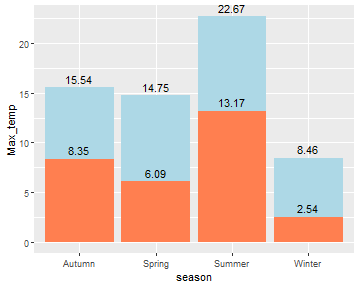
\includegraphics{Question-2_files/figure-latex/Figure3-1} 

}

\caption{Average Season Temperature \label{Figure3}}\label{fig:Figure3}
\end{figure}

The average maximum temperature in London is 22.67 degrees Celsius. My
word! This explains why everyone in London flocks to the beach when they
have ``good weather'' in the Summer.

The average temperatures can be enjoyed in Cape Town:\\
+ Summer: 20-30 degrees Celsius\\
+ Spring and Autumn: mid teens to mid 20's\\
+ Winter: mid teens to low 20's

\hypertarget{conclusion}{%
\section{Conclusion}\label{conclusion}}

If this doesn't convince you stay in Cape Town, then I don't know what
else will. You want to go based on your belief that it is sunnier, but I
hope this has shed some more light to what you can expect.

\begin{quote}
If you do go, at least enjoy the English Premier League
\end{quote}

\bibliography{Tex/ref}





\end{document}
